\section{Main Interface Screens}
\label{sec:main_interface_screens}%

In this chapter the User Interface for the application will be presented and explained in detail. Some changes have been made compared with the RASD, and some screens have been added for a more in-depth presentation.

\subsubsection{Main User Interface}

\begin{enumerate}
    \item \textbf{Main Dashboard Overview:} Features fast buttons to previous ratings and trips, and allows starting a new trip. The main screen provides quick access to all key features of the application. If the user is not registered, the buttons will lead to the registration form. There is also a button in the top right that directly accesses the user's profile, together with their statistics and data.
    \item \textbf{Path selection:} When a path is selected, its data is displayed. User may choose to start the ride if he's nearby or to see it's ratings clicking the button.
    \item \textbf{Path Search:} Search and visualize nearby bike paths or between origin and destination points.
   
\end{enumerate}

\begin{figure}[H]
    \centering
    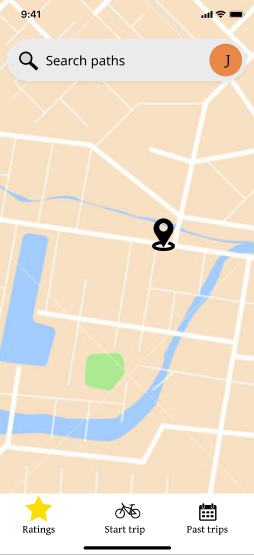
\includegraphics[width=0.3\linewidth]{Images/UI/main.png}\hfill
    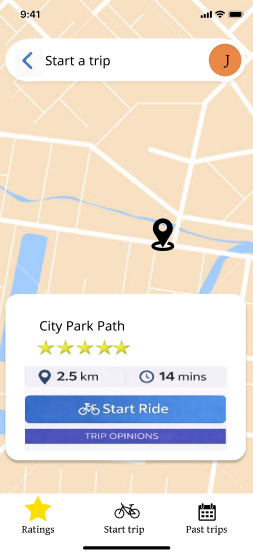
\includegraphics[width=0.3\linewidth]{Images/UI/start_trip.png}\hfill
    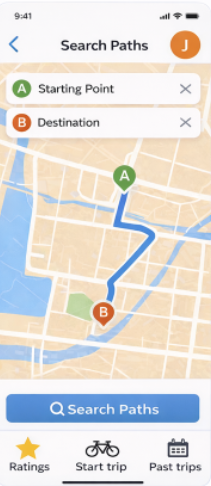
\includegraphics[width=0.3\linewidth, keepaspectratio=true]{Images/UI/search_paths.png}\hfill
    \caption{Here we see the interface of the main screen of the application and the interface when a certain path is selected.}
    \label{fig:ui_overview}
\end{figure}

\subsubsection{Settings and user data screen}

This screen provides access to users to their profile information and application settings. Users can view their personal statistics, including total distance traveled, number of trips completed, and cycling activity summary. The interface allows users to manage their account settings, update personal information, and configure application preferences such as notification settings.

\begin{figure}[H]
  \begin{center}
     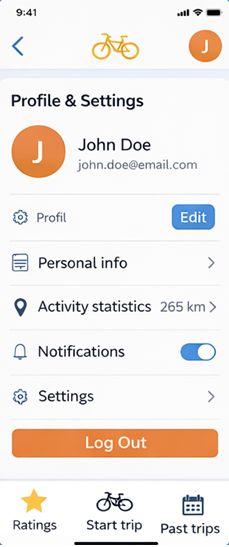
\includegraphics[width=0.35\linewidth, keepaspectratio=true]{Images/UI/profile.png}
     \caption{Profile settings and statistics screen.}
     \label{fig:profile_ui}%
  \end{center}
\end{figure}

\subsubsection{Trips and reviews interface}

\textbf{Screens overview:} The following screens show listings of trips and reviews. The user can select any of them by clicking. This will show more data about each rating/trip.

\begin{figure}[H]
    \centering
    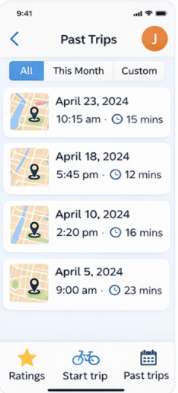
\includegraphics[width=0.3\linewidth, keepaspectratio=true]{Images/UI/past_trips.png}\hfill
    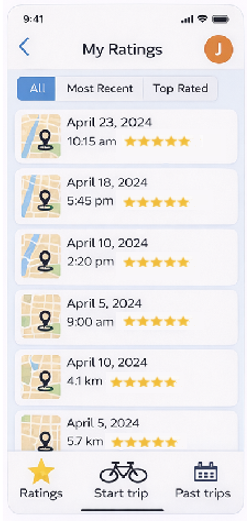
\includegraphics[width=0.3\linewidth, keepaspectratio=true]{Images/UI/my_ratings.png}\hfill
    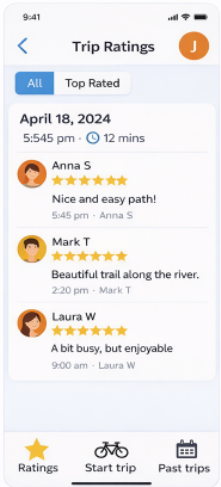
\includegraphics[width=0.3\linewidth, keepaspectratio=true]{Images/UI/trip_ratings.png}\hfill
    \caption{Here we see the interface of the main screen of the application and the interface when a certain path is selected.}
    \label{fig:ui_overview}
\end{figure}
  
